\documentclass[boxes]{homework}

% This is a slightly-more-than-minimal document that uses the homework class.
% See the README at http://git.io/vZWL0 for complete documentation.

\name{傅申 PB20000051}        % Replace (Your Name) with your name.
\term{2022 春}     % Replace (Current Term) with the current term.
\course{随机过程 B}    % Replace (Course Name) with the course name.
\hwnum{3}          % Replace (Number) with the number of the homework.
\hwname{作业}    
\problemname{习题}    
\solutionname{解:}

% Load any other packages you need here.
\usepackage[
    a4paper,
    top    = 2.4cm,
    bottom = 2.4cm,
    left   = 1.91cm,
    right  = 1.91cm,
    includeheadfoot
]{geometry}
\fancyfootoffset{0pt} % make fancyhdr work properly
\usepackage{ctex}
\usepackage{nicematrix}
\usepackage{tikz}
\usetikzlibrary{arrows,shapes,chains}

\begin{document}
\setlength\abovedisplayskip{.3em}
\setlength\belowdisplayskip{.3em}
\problemnumber{3}
\begin{problem}
信号传送问题. 信号只有 0, 1 两种, 分为多个阶段传输. 在每一步上出错的概率为 $\alpha$, $X_0 = 0$ 是送出的信号, 而
$X_n$  是在第 $n$ 步接受到的信号. 假定 $X_n$ 为一 Markov 链, 它有转移概率矩阵 $P_{00}=P_{11}=1-\alpha$,
$P_{01} =P_{10}=\alpha$, $0<\alpha<1$. 试求:
\begin{parts}[a]
    \part\label{3.a} 两步均不出错的概率 $P\{X_0 = 0, X_1 = 0, X_2 = 0\}$;
    \part\label{3.b} 两步传送后收到正确信号的概率;
    \part\label{3.c} 五步之后传送无误的概率 $P\{X_5 = 0\vert X_0 = 0\}$.
\end{parts}
\end{problem}

\begin{solution}
    \ref{3.a} 所求概率为
    \begin{equation}
        \begin{aligned}
            P\{X_0 = 0, X_1 = 0, X_2 = 0\}
             & = P\{X_2 = 0 \vert X_0 = 0, X_1 = 0\} P\{X_1 = 0 \vert X_0 = 0\} \\
             & = P\{X_2 = 0 \vert X_1 = 0\} P_{00}                              \\
             & = P_{00}^2                                                       \\
             & = \left(1 - \alpha\right)^2
        \end{aligned}
    \end{equation}

    \ref{3.b} 两步传送后收到正确信号的概率即为 $P^{(2)}_{00}$, 而有
    \begin{equation}
        \boldsymbol{P}^{(2)}
        = \begin{pmatrix}
            P^{(2)}_{00} & P^{(2)}_{01} \\
            P^{(2)}_{10} & P^{(2)}_{11}
        \end{pmatrix}
        = \boldsymbol{P}^{2}
        = \begin{pmatrix}
            1 - \alpha & \alpha     \\
            \alpha     & 1 - \alpha
        \end{pmatrix}^2
        = \begin{pmatrix}
            1 - 2\alpha + 2\alpha^2 & 2\alpha - 2\alpha^2     \\
            2\alpha - 2\alpha^2     & 1 - 2\alpha + 2\alpha^2
        \end{pmatrix}
    \end{equation}
    所以 $P^{(2)}_{00} = 1 - 2\alpha + 2\alpha^2$, 即两步传送后收到正确信号的概率为 $1 - 2\alpha + 2\alpha^2$.

    \ref{3.c} 五步之后传送无误的概率 $P\{X_5 = 0\vert X_0 = 0\} = P^{(5)}_{00}$, 而有
    \begin{equation}
        \boldsymbol{P}^{(5)}
        = \begin{pmatrix}
            P^{(5)}_{00} & P^{(5)}_{01} \\
            P^{(5)}_{10} & P^{(5)}_{11}
        \end{pmatrix}
        = \boldsymbol{P}^{5}
        = \begin{pmatrix}
            1 - \alpha & \alpha     \\
            \alpha     & 1 - \alpha
        \end{pmatrix}^5
    \end{equation}
    注意到
    \begin{equation}
        \boldsymbol{P}
        = \boldsymbol{T}^{-1} \begin{pmatrix}
            1 & 0           \\
            0 & 1 - 2\alpha
        \end{pmatrix} \boldsymbol{T}
        \qquad
        \boldsymbol{T}
        = \frac{1}{\sqrt{2}} \begin{pmatrix}
            1  & 1 \\
            -1 & 1
        \end{pmatrix},
        \boldsymbol{T}^{-1}
        = \frac{1}{\sqrt{2}} \begin{pmatrix}
            1 & -1 \\
            1 & 1
        \end{pmatrix}
    \end{equation}
    所以
    \begin{equation}
        \begin{aligned}
            \boldsymbol{P}^{(5)}
             & = \boldsymbol{T}^{-1} \begin{pmatrix}
                                         1 & 0           \\
                                         0 & 1 - 2\alpha
                                     \end{pmatrix}^5 \boldsymbol{T}
            = \boldsymbol{T}^{-1} \begin{pmatrix}
                                      1 & 0               \\
                                      0 & (1 - 2\alpha)^5
                                  \end{pmatrix} \boldsymbol{T}         \\
             & = \frac{1}{2} \begin{pmatrix}
                                 1 + (1 - 2\alpha)^5 & 1 - (1 - 2\alpha)^5 \\
                                 1 - (1 - 2\alpha)^5 & 1 + (1 - 2\alpha)^5
                             \end{pmatrix}
        \end{aligned}
    \end{equation}
    就有
    \begin{equation}
        P\{X_5 = 0\vert X_0 = 0\} = P^{(5)}_{00} = \frac{1}{2} \left[1 + (1 - 2\alpha)^5\right]
    \end{equation}
\end{solution}
\newpage
\problemnumber{5}
\begin{problem}
重复掷币一直到连续出现两次正面为止. 假定钱币是均匀的, 试引入以连续出现次数为状态空间的 Markov 链, 并求出平均需要掷多少次
试验才可以结束.
\end{problem}
\begin{solution}
    记 $X_n$ 为第 $n$ 次投掷连续出现正面的次数, 因为连续出现两次正面后试验就停止了, 所以状态空间为
    $\mathcal{X} = \{0, 1, 2\}$, 并且状态 2 为吸收态. 显然 $X_n$ 满足 Markov 性质如下:
    \begin{equation}
        \begin{gathered}
            P\{X_{n + 1} = 0 \vert X_0 = i_0, \cdots, X_{n - 1} = i_{n - 1}, X_n = i\}
            = P\{X_{n + 1} = 0 \vert X_n = i\} = \begin{cases}
                \frac{1}{2} & i = 0, 1 \\
                0           & i = 2
            \end{cases}\\
            P\{X_{n + 1} = 1 \vert X_0 = i_0, \cdots, X_{n - 1} = i_{n - 1}, X_n = i\}
            = P\{X_{n + 1} = 1 \vert X_n = i\} = \begin{cases}
                \frac{1}{2} & i = 0    \\
                0           & i = 1, 2
            \end{cases}\\
            P\{X_{n + 1} = 2 \vert X_0 = i_0, \cdots, X_{n - 1} = i_{n - 1}, X_n = i\}
            = P\{X_{n + 1} = 2 \vert X_n = i\} = \begin{cases}
                0           & i = 0 \\
                \frac{1}{2} & i = 1 \\
                1           & i = 2
            \end{cases}
        \end{gathered}
    \end{equation}
    所以 $\{X_n, n = 0, 1, \cdots\}$ 为 Markov 链, 状态转移矩阵如下:
    \begin{equation}
        \boldsymbol{P} = \begin{pmatrix}
            \frac{1}{2} & \frac{1}{2} & 0           \\
            \frac{1}{2} & 0           & \frac{1}{2} \\
            0           & 0           & 1
        \end{pmatrix}
    \end{equation}
    令 $X_0 = 0$, 这就与试验中的情况相同. 记 $T = \min\{n \ge 0 \vert X_n = 2\}$, 要求平均需要掷多少次试验才可
    以结束, 即求 $u = E\{T \vert X_0 = 0\}$. 可以建立关于 $u$ 的方程如下:
    \begin{equation} \label{eq:5.3}
        \begin{aligned}
            u & = \sum_{k = 0}^2 E\{T \vert X_0 = 1, X_1 = k\} P\{X_1 = k \vert X_0 = 0\} \\
              & = \sum_{k = 0}^2 E\{T \vert X_1 = k\} P\{X_1 = k \vert X_0 = 0\}          \\
              & = \frac{1}{2} \left[E\{T\vert X_1 = 0\} + E\{T\vert X_1 = 1\}\right]      \\
              & = \frac{1}{2} \left[(u + 1) + (v + 1)\right]                              \\
              & = \frac{1}{2} \left(u + v\right) + 1
        \end{aligned}
    \end{equation}
    其中 $v = E\{T \vert X_0 = 1\}$, 建立关于其的方程如下:
    \begin{equation} \label{eq:5.4}
        \begin{aligned}
            v & =  \sum_{k = 0}^2 E\{T \vert X_1 = k\} P\{X_1 = k \vert X_0 = 1\}    \\
              & = \frac{1}{2} \left[E\{T\vert X_1 = 0\} + E\{T\vert X_1 = 2\}\right] \\
              & = \frac{1}{2} \left[(u + 1) + 1\right]                               \\
              & = \frac{1}{2} u + 1
        \end{aligned}
    \end{equation}
    联立方程 (\ref{eq:5.3}) 和 (\ref{eq:5.4}) 解得 $u = 6$ 和 $v = 4$. 因此平均需要掷 $6$ 次试验才可以结束.
\end{solution}

\problemnumber{8}
\begin{problem}
记 $Z_i, i = 1, 2, \cdots$ 为一串独立同分布的离散随即变量. $P\{Z_1 = k\} = p_k \ge 0, k = 0, 1, 2, \cdots$, \
$\displaystyle \sum_{k = 0}^\infty p_k = 1$. 令 $X_n = \max\{Z_1, \cdots, Z_n\}, n = 1,
    2, \cdots$, 并约定 $X_0 = 0$. $X_n$ 是否为 Markov 链? 如果是, 其转移概率阵是什么?
\end{problem}
\begin{solution}
    由题意可知, $\{X_n, n = 0, 1, \cdots\}$ 的状态空间为 $\mathcal{X} = \mathbb{N}$. 因为
    $X_n = \max\{Z_1, \cdots, Z_n\}, n = 1, 2, \cdots$, 所以有 $X_{n + 1} = \max\{X_n, Z_{n + 1}\}$,
    且 $X_n, Z_{n + 1}, Z_{n + 2}, \cdots$ 独立. 对任意的 $n \ge 0$ 和任意
    $i_1, \cdots, i_{n - 1}, i, j \in \mathcal{X}$, 有
    \begin{equation}
        \begin{aligned}
            P\{X_{n + 1} = j \vert X_0 = 0, X_1 = i_1, \cdots, X_n = i\}
             & = P\{\max\{X_n, Z_{n + 1}\} = j \vert X_0 = 0, X_1 = i_1, \cdots, X_n = i\} \\
             & = P\{\max\{X_n, Z_{n + 1}\} = j \vert X_n = i\}                             \\
             & = P\{X_{n + 1} = j \vert X_n = i\}
        \end{aligned}
    \end{equation}
    所以 $\{X_n, n \ge 0\}$ 满足 Markov 性质, $X_n$ 为 Markov 链. 其转移概率为
    \begin{equation}
        P_{ij} = P\{X_{n + 1} = j \vert X_n = i \} = \begin{cases}
            0                                         & j < i \\
            P\{Z_{n + 1} \le i\} = \sum_{k = 0}^i p_k & j = i \\
            P\{Z_{n + 1} = j\} = p_j                  & j > i
        \end{cases}
    \end{equation}
    所以 $X_n$ 的转移概率阵为
    \begin{equation}
        \boldsymbol{P} = \begin{pmatrix}
            p_0    & p_1       & p_2             & p_3                   & \cdots \\
            0      & p_0 + p_1 & p_2             & p_3                   & \cdots \\
            0      & 0         & p_0 + p_1 + p_2 & p_3                   & \cdots \\
            0      & 0         & 0               & p_0 + p_1 + p_2 + p_3 & \cdots \\
            \vdots & \vdots    & \vdots          & \vdots                & \ddots \\
        \end{pmatrix}
    \end{equation}
\end{solution}

\problemnumber{11}
\begin{problem}
一 Markov 链有状态 0, 1, 2, 3 和转移概率矩阵
$$
    \boldsymbol{P} = \begin{pmatrix}
        0           & \frac{1}{2} & 0 & \frac{1}{2} \\
        0           & 0           & 1 & 0           \\
        0           & 0           & 0 & 1           \\
        \frac{1}{2} & 0           & 0 & \frac{1}{2}
    \end{pmatrix}
$$
试求 $f_{00}^{(n)}, n = 1, 2, 3, 4, 5, \cdots$, 其中 $f_{ii}^{(n)} = P\{X_n = i, X_k \neq i,
    k = 1, \cdots, n - 1 \vert X_0 = i\}$.
\end{problem}
\begin{solution}
    首先, $f_{00}^{(1)} = P_{00} = 0$.

    对 $n \ge 2$, 定义方阵 $\boldsymbol{P}'$
    \begin{equation}
        \boldsymbol{P}' = \begin{pmatrix}
            0           & 0 & 0 & 0           \\
            0           & 0 & 1 & 0           \\
            0           & 0 & 0 & 1           \\
            \frac{1}{2} & 0 & 0 & \frac{1}{2}
        \end{pmatrix}
    \end{equation}
    即原 Markov 链的状态 0 不会转移再到任何状态, 在下个时间就此消失. 那么 $f_{(00)}^{(n)}$ 就是
    $\boldsymbol{P}_0{\boldsymbol{P}'}^{n - 1}$ 的第一个元素. 其中 $\boldsymbol{P}_0 =
        (0, \frac{1}{2}, 0, \frac{1}{2})$ 为 $X_1$ 的概率向量.

    下面计算 ${\boldsymbol{P}'}^{n - 1}$, 注意到 $\boldsymbol{P}'$ 的特征多项式为 $\det(\lambda
        \boldsymbol{I} - \boldsymbol{P}') = \lambda^4 - \frac{1}{2}\lambda^3$, 所以有
    ${\boldsymbol{P}'}^4 = \frac{1}{2}{\boldsymbol{P}'}^3$, 因此只需要求出 $\boldsymbol{P}'$ 的 1, 2,
    3 次幂即可, 如下:
    \begin{equation}
        {\boldsymbol{P}'}^1 = \boldsymbol{P}' = \begin{pmatrix}
            0           & 0 & 0 & 0           \\
            0           & 0 & 1 & 0           \\
            0           & 0 & 0 & 1           \\
            \frac{1}{2} & 0 & 0 & \frac{1}{2}
        \end{pmatrix}
        \qquad
        {\boldsymbol{P}'}^2 = \begin{pmatrix}
            0           & 0 & 0 & 0           \\
            0           & 0 & 0 & 1           \\
            \frac{1}{2} & 0 & 0 & \frac{1}{2} \\
            \frac{1}{4} & 0 & 0 & \frac{1}{4}
        \end{pmatrix}
        \qquad
        {\boldsymbol{P}'}^3 = \begin{pmatrix}
            0           & 0 & 0 & 0           \\
            \frac{1}{2} & 0 & 0 & \frac{1}{2} \\
            \frac{1}{4} & 0 & 0 & \frac{1}{4} \\
            \frac{1}{8} & 0 & 0 & \frac{1}{8}
        \end{pmatrix}
    \end{equation}
    那么就得到
    \begin{equation}
        {\boldsymbol{P}'}^n = \begin{pmatrix}
            0         & 0 & 0 & 0         \\
            2^{2 - n} & 0 & 0 & 2^{2 - n} \\
            2^{1 - n} & 0 & 0 & 2^{1 - n} \\
            2^{- n}   & 0 & 0 & 2^{- n}   \\
        \end{pmatrix}
        \quad , n \ge 3
    \end{equation}
    对 $n \ge 2$ 求 $\boldsymbol{P}_0{\boldsymbol{P}'}^{n - 1}$ 的第一个元素, 进而求 $f_{(00)}^{(n)}$,
    得到下面的结果:
    \begin{align}
        f_{00}^{(1)} & = 0                                                       \\
        f_{00}^{(2)} & = \left(0, \frac{1}{2}, 0, \frac{1}{2}\right)
        \left(0, 0, 0, \frac{1}{2}\right)^T = \frac{1}{4}                        \\
        f_{00}^{(3)} & = \left(0, \frac{1}{2}, 0, \frac{1}{2}\right)
        \left(0, 0, \frac{1}{2}, \frac{1}{4}\right)^T = \frac{1}{8}              \\
        f_{00}^{(4)} & = \left(0, \frac{1}{2}, 0, \frac{1}{2}\right)
        \left(0, \frac{1}{2}, \frac{1}{4}, \frac{1}{8}\right)^T = \frac{5}{16}   \\
        f_{00}^{(5)} & = \left(0, \frac{1}{2}, 0, \frac{1}{2}\right)
        \left(0, \frac{1}{4}, \frac{1}{8}, \frac{1}{16}\right)^T = \frac{5}{32}  \\
        f_{00}^{(n)} & = 2^{-(n - 4)}f_{00}^{(4)} = \frac{5}{2^n}, \quad n \ge 4
    \end{align}
\end{solution}

\problemnumber{13}
\begin{problem}
试证向各方向游动的概率相等的对称随机游动在二维时是常返的, 而在三维时却是瞬过的.
\end{problem}
\begin{solution}
    先考虑二维情形. 设 $X_n, n \ge 0$ 为二维对称随机游动的 Markov 链, 则其状态空间为 $\mathcal{X} = \mathbb{Z}^2$.
    显然这个 Markov 链是不可约的, 所以我们只需要考虑状态 0 (即原点) 的常返性. 记向上下左右方向移动的次数为 $k_{n,1}$,
    $k_{n,2}$, $k_{n,3}$, $k_{n,4}$, 那么 $\boldsymbol{k}_n = (k_{n,1}, k_{n,2}, k_{n,3}, k_{n,4})$
    服从多项分布, 且 $X_n = (k_{n,1} - k_{n,2}, k_{n,3} - k_{n,4})$, 那么就有
    \begin{equation}
        P_{00}^{(n)} = P\{k_{n,1} = k_{n,2}, k_{n,3} = k_{n,4}\}
    \end{equation}
    显然 $n$ 为奇数时上面的式子结果为 0, 所以我们只考虑 $n$ 为偶数的情况. 如下
    \begin{equation}
        \begin{aligned}
            P_{00}^{(2n)}
             & = P\{k_{2n,1} = k_{2n,2}, k_{2n,3} = k_{2n,4}\}
            = \sum_{i = 0}^n P\{k_{2n,1} = k_{2n,2} = i, k_{2n,3} = k_{2n,4} = n - i\} \\
             & = \sum_{i = 0}^n \frac{(2n)!}{i! i! (n - i)! (n - i)!}\frac{1}{4^{2n}}
            = \frac{1}{4^{2n}}\mathrm{C}_{2n}^n \sum_{i = 0}^n \mathrm{C}_{n}^i \mathrm{C}_{n}^{n - i}
            = \frac{1}{4^{2n}}\left(\mathrm{C}_{2n}^n\right)^2
            = \frac{1}{4^{2n}}\left[\frac{(2n)!}{(n!)^2}\right]^2
        \end{aligned}
    \end{equation}
    由 Stirling 公式, 有
    \begin{equation}
        P_{00}^{(2n)} = \frac{1}{4^{2n}}\left[\frac{(2n)!}{(n!)^2}\right]^2 \sim
        \frac{1}{4^{2n}}\left[\frac{2^{2n}}{\sqrt{n\pi}}\right]^2 = \frac{1}{n\pi}
    \end{equation}
    而 $\sum_{n = 1}^\infty \frac{1}{n\pi} = \infty$, 所以有
    \begin{equation}
        \sum_{n = 0}^\infty P_{00}^{(n)} = \sum_{n = 0}^\infty P_{00}^{(2n)} = \infty
    \end{equation}
    因此, 状态 0 是常返的, 进而二维对称随机游动是常返的.

    然后考虑三维情况, 类似地, 在三维情况下 Markov 链不可约, 只考虑状态 0 (原点) 的常返性.\\
    $n$ 为奇数时, $P_{00}^{(n)} = 0$; 为偶数时, 有
    \begin{equation}
        P_{00}^{(2n)}
        = \sum_{i = 0}^n\sum_{j = 0}^{n - i}
        \frac{(2n)!}{i! i! j! j! (n - i - j)! (n - i - j)!}\frac{1}{6^{2n}}
        = \frac{1}{6^{2n}}\mathrm{C}_{2n}^n \sum_{i = 0}^n\sum_{j = 0}^{n - i}
        \left[\frac{n!}{i! j! (n - i - j)!}\right]^2
    \end{equation}
    若 $n = 3m$, 有
    \begin{equation}
        \begin{aligned}
            P_{00}^{(6m)}
             & \le \frac{1}{6^{6m}}\mathrm{C}_{6m}^{3m} \sum_{i = 0}^{3m}\sum_{j = 0}^{3m - i}
            \frac{(3m)!}{i! j! (3m - i - j)!}\frac{(3m)!}{m!m!m!}                                   \\
             & = \frac{1}{2^{6m}\times 3^{3m}}\mathrm{C}_{6m}^{3m}\frac{(3m)!}{m!m!m!}
            \sum_{i = 0}^{3m}\sum_{j = 0}^{3m - i}\frac{(3m)!}{i! j! (3m - i - j)!}\frac{1}{3^{3m}} \\
             & = \frac{1}{2^{6m}\times 3^{3m}}\mathrm{C}_{6m}^{3m}\frac{(3m)!}{m!m!m!}              \\
             & \sim \frac{1}{2^{6m}\times 3^{3m}} \left[\frac{2^{6m}}{\sqrt{3m\pi}}\right]
            \left[\frac{\sqrt{3}\times 3^{3m}}{2m\pi}\right]                                        \\
             & \sim \left(\frac{1}{m\pi}\right)^{3/2}
        \end{aligned}
    \end{equation}
    而当 $n = 3m - 1$ 时, 有
    \begin{equation}
        \begin{aligned}
            P_{00}^{(6m)}
             & = P\{X_{6m} = 0\}                                          \\
             & \ge P\{X_{6m} = 0, X_{6m - 2} = 0\}                        \\
             & = P\{X_{6m} = 0 \vert X_{6m - 2} = 0\} P\{X_{6m - 2} = 0\} \\
             & = P_{00}^{(2)} P_{00}^{(6m - 2)}                           \\
             & = \frac{1}{6} P_{00}^{(6m - 2)}
        \end{aligned}
    \end{equation}
    所以 $P_{00}^{(6m - 2)} \le 6 P_{00}^{(6m)}$, 同理有 $P_{00}^{(6m - 4)} \le 6 P_{00}^{(6m -2)} \le
        36 P_{00}^{(6m)}$.\\
    因为 $\sum_{m = 1}^\infty \left(\frac{1}{m\pi}\right)^{3/2} < \infty$, 所以有
    \begin{equation}
        \sum_{n = 0}^\infty P_{00}^{(n)} \le \sum_{m = 1}^\infty (1 + 6 + 36)P_{00}^{(6m)} < \infty
    \end{equation}
    因此, 状态 0 是瞬过的, 进而三维对称随机游动是瞬过的.
\end{solution}
\newpage
\problemnumber{18}
\begin{problem}
假定在逐日的天气变化模型中, 每天的阴晴与前两天的状况关系很大. 于是可考虑 4 状态的 Markov 链: 接连两晴天, 一晴一阴,
一阴一晴, 以及接连两阴天, 分别记为 $(S,S)$, $(S,C)$, $(C,S)$ 和 $(C,C)$. 该链的转移概率阵为
\begin{equation}
    \boldsymbol{P} =
    \begin{pNiceMatrix}[first-row, first-col]
              & (S,S) & (S,C) & (C,S) & (C,C) \\
        (S,S) & 0.8   & 0.2   & 0     & 0     \\
        (S,C) & 0     & 0     & 0.4   & 0.6   \\
        (C,S) & 0.6   & 0.4   & 0     & 0     \\
        (C,C) & 0     & 0     & 0.1   & 0.9
    \end{pNiceMatrix}
\end{equation}
试求这一 Markov 链的平稳分布. 并求出长期平均的晴朗天数.
\end{problem}
\begin{solution}
    该 Markov 链的状态转移图如下:
    \begin{center}
        \resizebox{0.35\textwidth}{!}{
            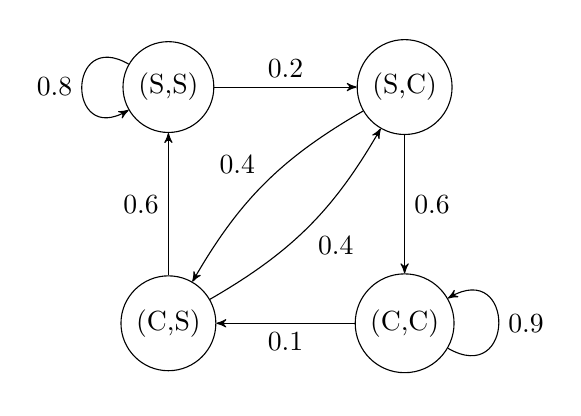
\begin{tikzpicture}[
                    ->,
                    >=stealth',
                    align = center,
                    auto,
                    node distance=3cm,
                    node/.style = {draw, circle, fill = none, minimum size = 1cm}]
                \node[node]               (1) {(S,S)};
                \node[node, right of = 1] (2) {(S,C)};
                \node[node, below of = 1] (3) {(C,S)};
                \node[node, right of = 3] (4) {(C,C)};
                \path[]
                (1) edge [out = 150, in = 210, looseness = 4] node [left]        {0.8} (1)
                (1) edge                                      node [above]       {0.2} (2)
                (2) edge [bend right = 15]                    node [above left]  {0.4} (3)
                (2) edge                                      node [right]       {0.6} (4)
                (3) edge                                      node [left]        {0.6} (1)
                (3) edge [bend right = 15]                    node [below right] {0.4} (2)
                (4) edge                                      node [below]       {0.1} (3)
                (4) edge [out = 330, in = 30, looseness = 4]  node [right]       {0.9} (4)
                ;
            \end{tikzpicture}
        }
    \end{center}
    说明 Markov 链是不可约的. 记四个状态分别为 1, 2, 3, 4, 求解下面的方程:
    \begin{gather}
        \sum_{j = 1}^4 \pi_j = 1, \pi_j > 0 \\
        \sum_{i = 1}^4 \pi_i P_{ij} = \pi_j
    \end{gather}
    可以解得唯一的
    \begin{equation}
        \pi = \{\pi_1, \pi_2, \pi_3, \pi_4\} =
        \left\{\frac{3}{11}, \frac{1}{11}, \frac{1}{11}, \frac{6}{11}\right\}
    \end{equation}
    此即为该 Markov 链的平稳分布, 所以长期平均的晴朗天数为
    \begin{equation}
        \frac{3}{11} + \frac{1}{11} \times \frac{1}{2} + \frac{1}{11} \times \frac{1}{2} = \frac{4}{11}
    \end{equation}
\end{solution}
\problemnumber{19}
\begin{problem}
某人有 $M$ 把伞并在办公室和家之间往返. 如某天他在家时 (办公室时) 下雨了而且家 (办公室) 有伞他就带一把伞去上班
(回家), 不下雨时他从不带伞. 如果每天与以往独立地早上 (或晚上) 下雨的概率为 $p$, 试定义一 $M+1$ 状态的 Markov 链
以研究他被雨淋湿的机会.
\end{problem}
\begin{solution}
    记 $X_n$ 为第 $n$ 天早晨家中的雨伞数, 则 $X_n$ 为 Markov 链, 状态空间为 $\mathcal{X} = \{0, 1, \cdots, M\}$. 
    记 $q = 1 - p$, 其状态转移矩阵可以写成下面的形式:
    
    \begin{equation}
        \boldsymbol{P} =
        \begin{pNiceMatrix}[first-row]
            0                      & 1         & 2         & \cdots & \cdots                 & M - 2     & M - 1     & M    \\
            q                      & p         &           &        & \Block{4-4}<\Large>{0}                                \\
            pq                     & p^2 + q^2 & pq        &        &                        &           &           &      \\
                                   & pq        & p^2 + q^2 & pq     &                        &           &           &      \\
                                   &           & \ddots    & \ddots & \ddots                 &           &           &      \\
            \Block{4-3}<\Large>{0} &           &           & \ddots & \ddots                 & \ddots    &           &      \\
                                   &           &           &        & pq                     & p^2 + q^2 & pq        &      \\
                                   &           &           &        &                        & pq        & p^2 + q^2 & pq   \\
                                   &           &           &        &                        &           & pq        & 1-pq \\
        \end{pNiceMatrix}
    \end{equation}
    显然这个 Markov 链是不可约的, 解下面的方程组:
    \begin{gather}
        \sum_{j = 0}^M \pi_j = 1, \pi_j > 0 \\
        \sum_{i = 0}^M \pi_i P_{ij} = \pi_j
    \end{gather}
    可以解得唯一的
    \begin{equation}
        \pi_0 = \frac{1 - p}{M + 1 - p}, \pi_1 = \pi_2 = \cdots = \pi_M = \frac{1}{M + 1 - p}
    \end{equation}
    $\pi = \{\pi_0, \pi_1, \cdots, \pi_M\}$ 即为 Markov 链的平稳分布, 所以他被雨淋湿的概率为
    \begin{equation}
        P\{\text{该人被雨淋湿}\} = p\pi_0 + qp\pi_M = \frac{2p (1 - p)}{M + 1 - p}
    \end{equation}
\end{solution}
\problemnumber{22}
\begin{problem}
若一单体产生后代的分布为 $p_0 = q$, $p_1 = p$ ($p + q = 1$), 并假定过程开始时的祖先数为 1, 试求分支过程第三代
总数的分布.
\end{problem}
\begin{solution}
    记 $X_n$ 为第 $n$ 代个体数, 并令 $X_0 = 1$, 则 $X_n$ 是 Markov 链, 且为分支过程, 其状态空间为
    $\mathcal{X} = \{0, 1\}$
    则前三代的生成函数为:
    \begin{align}
        \phi_1(s) & = E\left[s^{X_1}\right] = E\left[s^Z_1\right] = s^0p_0 + s^1p_1 = q + ps  \\
        \phi_2(s) & = \phi_1(\phi_1(s)) = \phi_1(q + ps) = q + pq + p^2 s = 1 - p^2 + p^2 s \\
        \phi_3(s) & = \phi_1(\phi_2(s)) = \phi_1(1 - p^2 + p^2 s) = q + p(1 - p^2 + p^2 s)
        = 1 - p^3 + p^3 s
    \end{align}
    因此就有
    \begin{equation}
        P\{X_3 = 0\} = E\left[0^{X_3}\right] = \phi_3(0) = 1 - p^3
        \qquad P\{X_3 = 1\} = 1 - P\{X_3 = 0\} = p^3
    \end{equation}
    即为第三代总数的分布
\end{solution}
\end{document}
